A continuación se muestran las diferentes vistas arquitectónicas que plasman los diagramas la Kiwi Platform.

\subsection{Vista de Descomposición}
La vista de descomposición encierra y describe toda nuestra aplicación en los siguientes módulos principales:
\begin{itemize}
    \item kwii-api:\\\\
    Este módulo es el responsable de orquestar los flujos de procesos de la plataforma. En él se encuentra la lógica del manejo de peticiones, redirigiendo el trabajo de todos los microservicios de la aplicación.
    
    \item Users\\\\
    El módulo de usuarios es el encargado de llevar la lógica de los usuarios, éste a su vez es dividido en los siguientes tres submódulos:
    \begin{itemize}
        \item user-ms \\\
        El microservicio de los usuarios, módulo encargado de almacenar y exponer la información de los usuarios. Este submódulo permite la administración de los perfiles de usuario ademas de relacionarlos entre ellos y guardar registros de los usuarios en el LDAP.
        \item authentication-ms \\\
        El microservicio de autenticación, permite a los usuarios tener sesiones dentro de la aplicación. Este microservicio es el principal para cuestiones de seguridad en la sesión de los usuarios en el sistema.
        \item kwii-ldap\\\
        El servicio ldap que traza información de los usuarios. Así como sus contraseñas.
    \end{itemize}
    
    \item Chats \\\\
    El módulo de chats es el gran módulo que vela por la creación de chats y la entrega de mensajes entre ellos, además también se encarga de notificar a los usuarios sobre el uso de estos chats. Este gran módulo se divide en los tres siguientes submódulos:
    \begin{itemize}
        \item chat-ms\\\
        El submódulo chat-ms es el encargado de almacenar y exponer información sobre los mensajes enviados en los chats de la aplicación.
        \item chatroom-ms\\\
        El submódulo chatroom-ms es el encargado de la gestión de los chats, los chats son los lugares donde se intercambian mensajes. Estos chats pueden ser consumidos por los usuarios asociados a esos chats.
        \item notifications-ms
        El submódulo encargado de la entrega de notificaciones a los usuarios es notification-ms, él vela por informar a los usuarios de la aplicación sobre el intercambio de mensajes de la aplicación.
    \end{itemize}

    \item Exposer\\\\
    El módulo Exposer es el módulo referente a la exposición de los servicios de la aplicación. Este módulo vela por la interacción de la aplicación con el exterior. Este módulo contiene los siguientes submódulos:
    \begin{itemize}
        \item kwii-interface\\\
        Este submodulo es el encargado de exponer funcionalidades de nuestra plataforma hacia otros sistemas de software,  a su vez se encarga de consumir servicios expuestos por otros sistemas.
        \item kwii-proxy\\\
        Este submódulo ofrece nuestros servicios a internet para que sean consumidos por usuarios a mayor escala.
    \end{itemize}

    \item Front End\\\\
    En el módulo de front end encerramos la funcionalidad de disponer al usuario de forma cómoda la información de nuestra aplicación. Éste módulo encierra dos grandes submódulos que se refieren a la fomra de presentar nuesta información:
    \begin{itemize}
        \item Web Client\\\
        Este submódulo se refiere a la funcionalidad de nuestra aplicación que expone nuestros servicios a usuarios que usan la plataforma por medio de un navegador web. 
        \item Mobile Client\\\
        Este submódulo se refiere a la funcionalidad de nuestra aplicación que expone nuestros servicios a usuarios que usan la plataforma por medio de un dispositivo móvil. 
    \end{itemize}
\end{itemize}

\begin{center}
    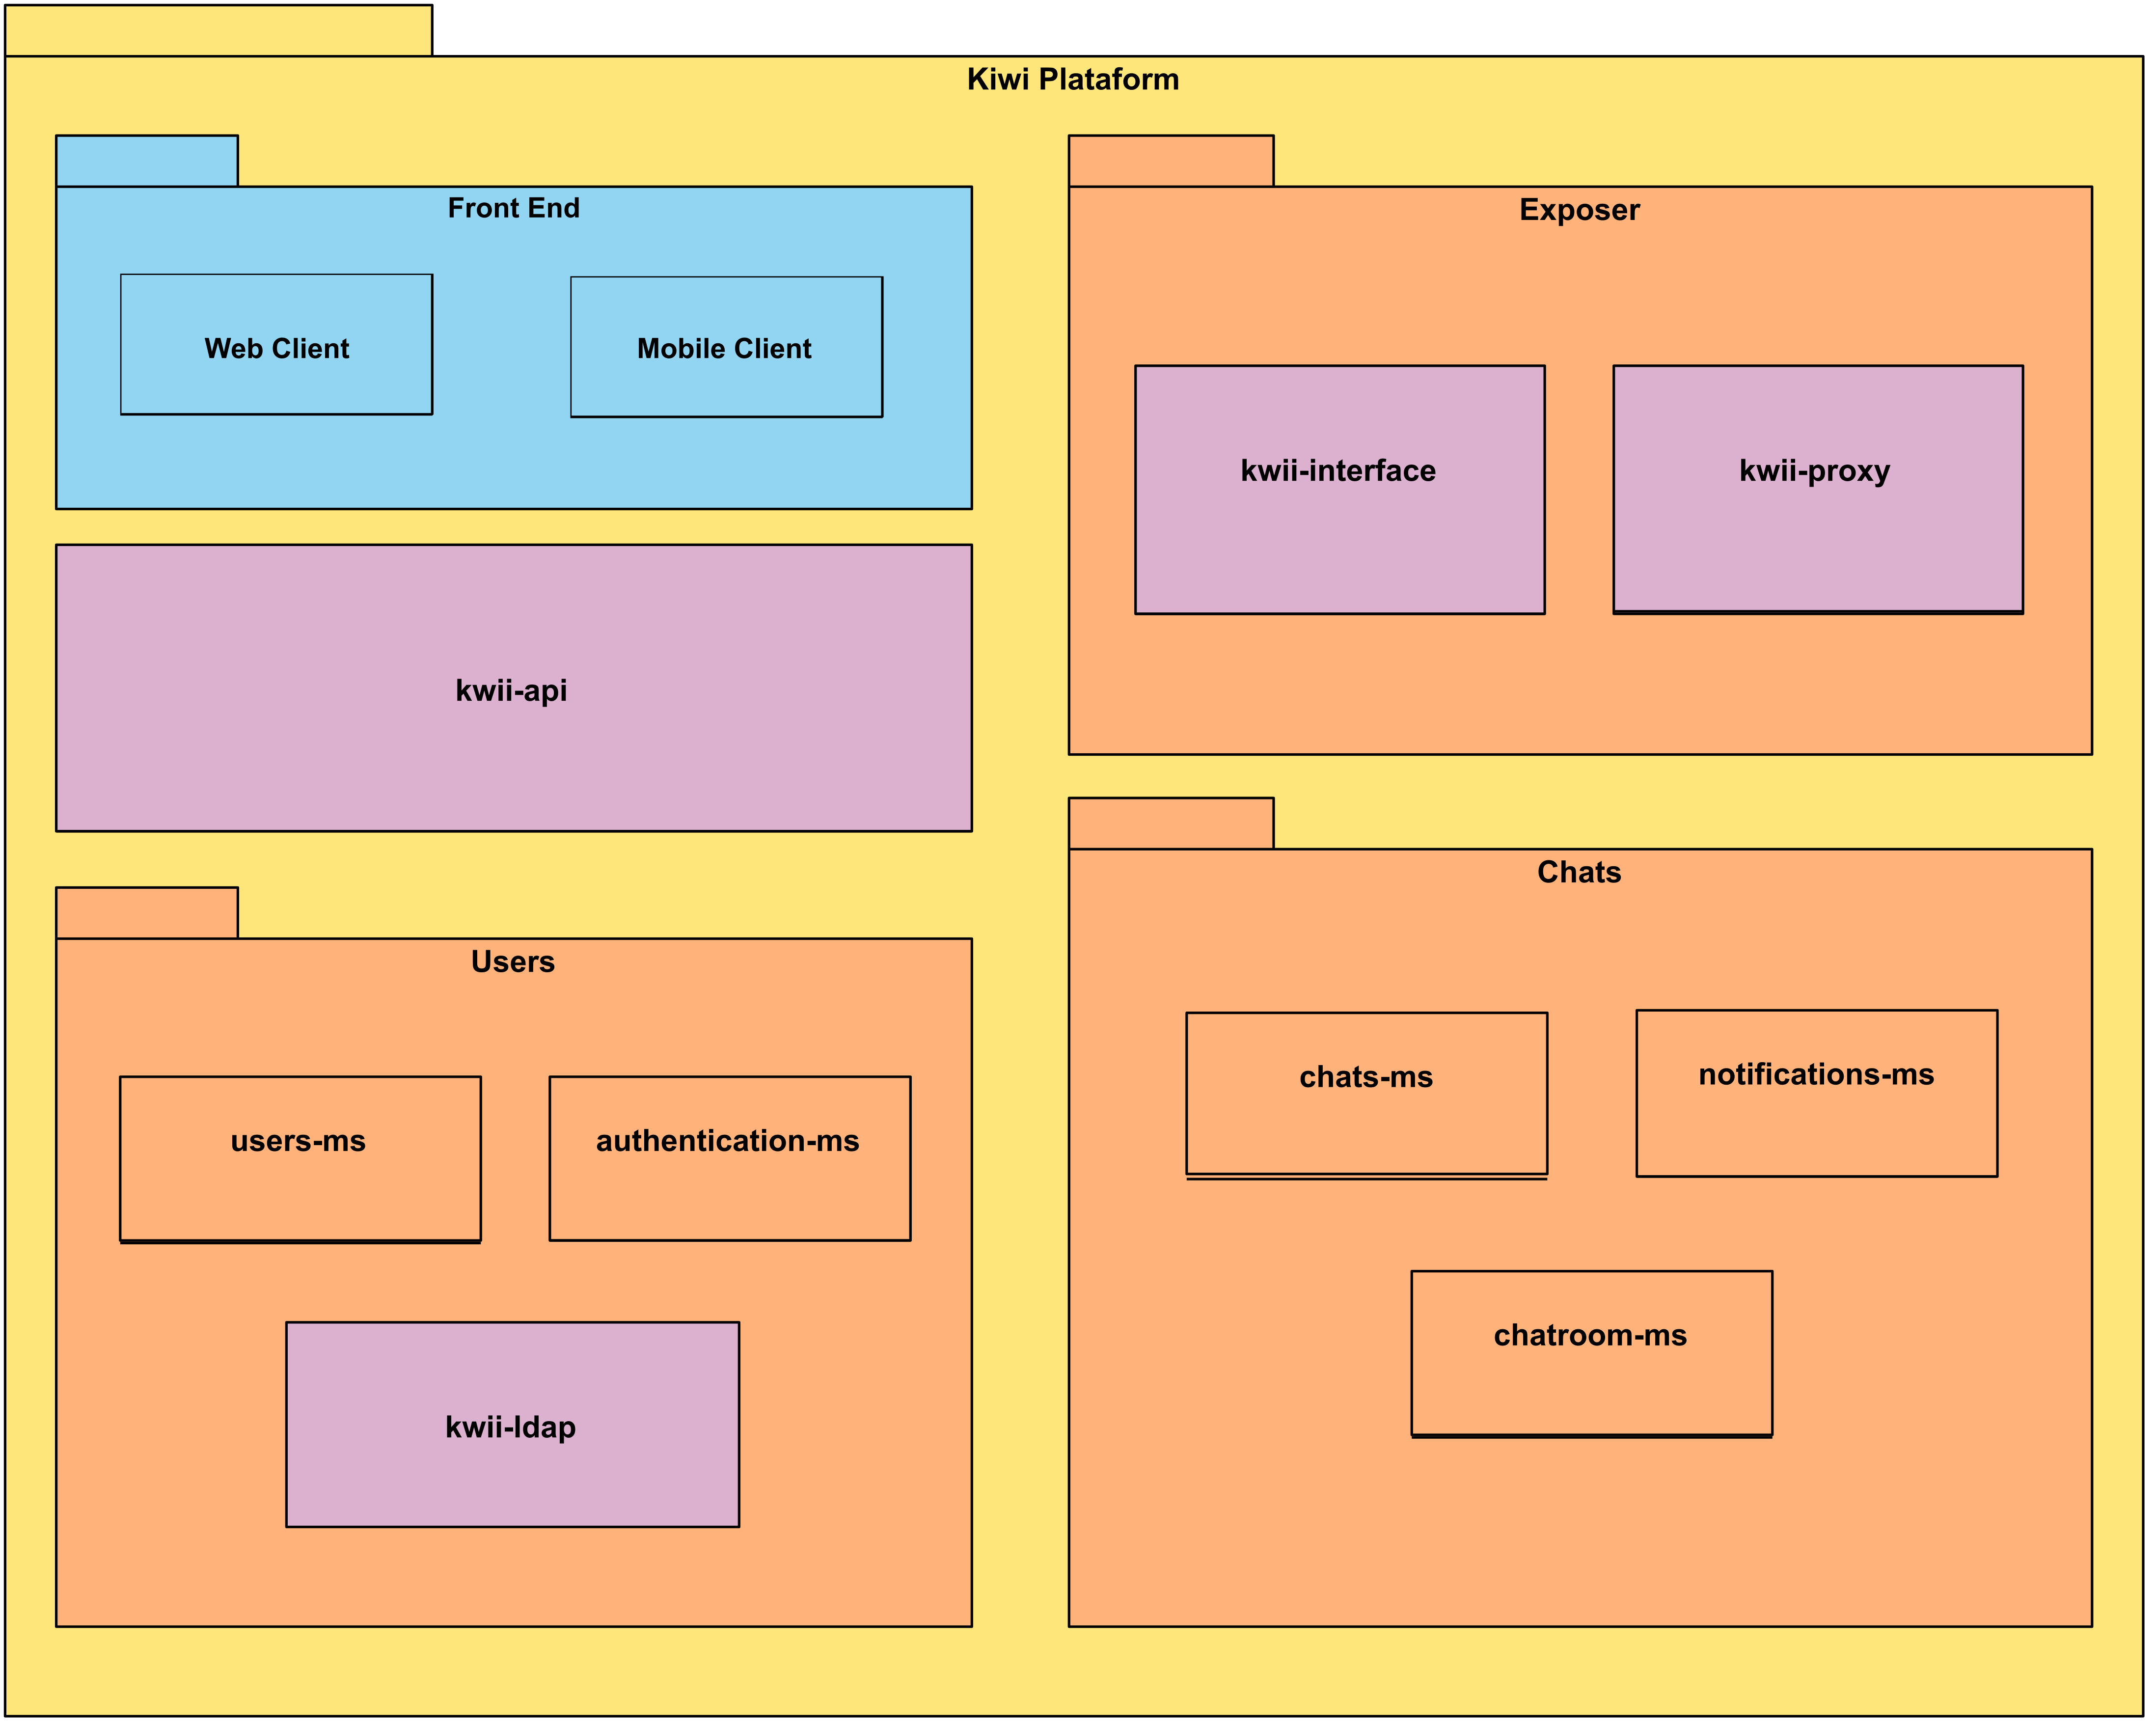
\includegraphics[width=16cm]{Figures/P3/Decomposition.png}  
\end{center}

\subsection{Vista de Modelos de Datos}
Las vistas de los modelos de datos nos muestra la aplicación desde la perspectiva de sus datos, y cómo residen ellos en nuestra aplicación. Se evidencia en los diagramas cómo cada microservicio de la aplicación es dueño de sus datos y los manipula y expone a su conveniencia.
\subsubsection{Microservicio usuarios}
En el modelo de datos del microservicio usuarios encontramos una estuctura en la que se guardan cosas relevantes referentes a ellos, tales como el nombre o su contraseña secreta. Esta estructura puede ser ampliada cuando sea necesario, para almacenar más información acerca de los usuarios. \\
Además se presenta una relación de muchos a muchos de los usuarios con ellos mismos, para trazar la información de los amigos de un usuario; de esta forma, un usuario puede tener muchos amigos, y muchos amigos (otros usuarios) pueden ser amigos de un mismo usuario.
\begin{center}
    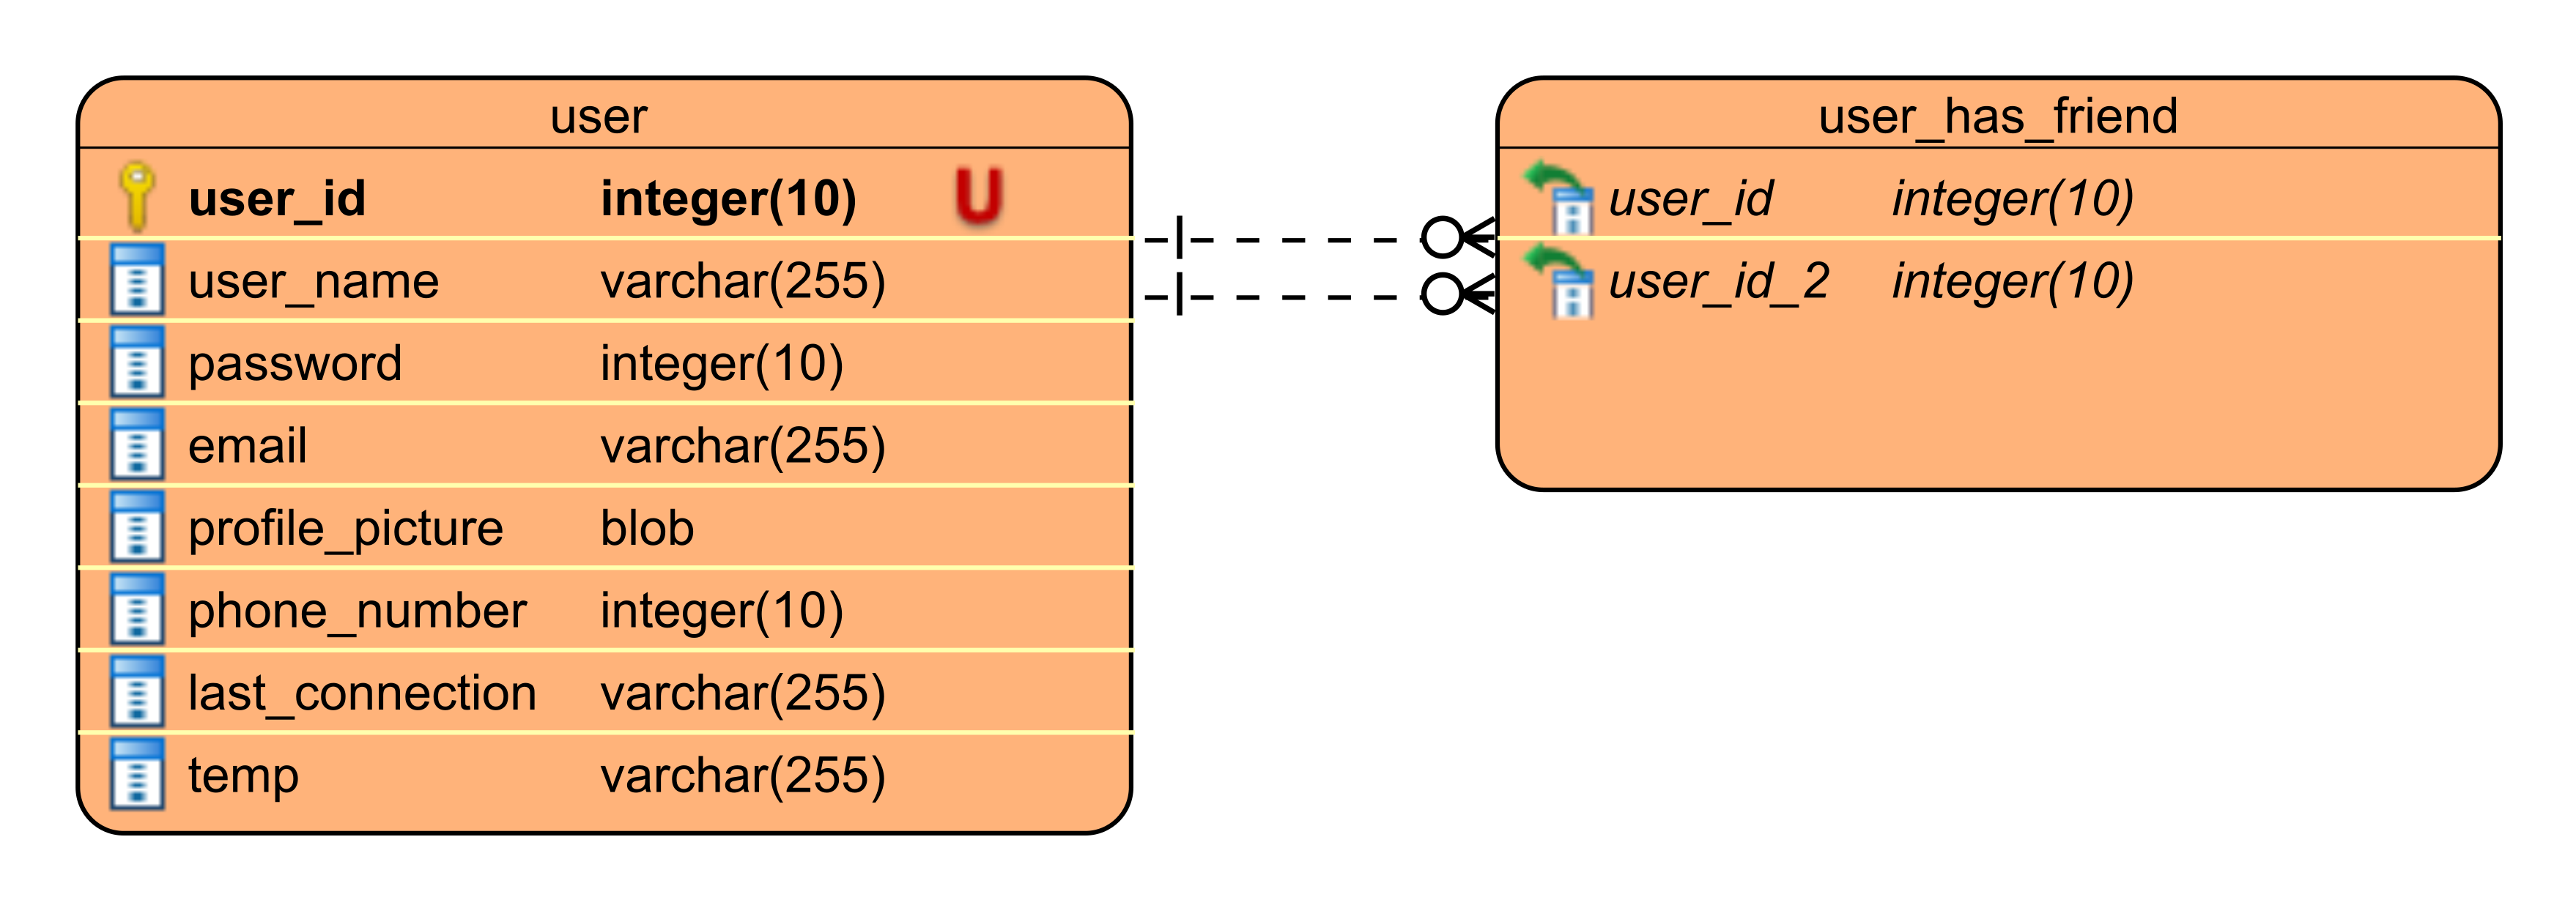
\includegraphics[width=9cm]{Figures/P3/DataModelUsers.png}    
\end{center}
\subsubsection{Microservicio autenticación}
En esta vista, mostramos que el microservicio de autenticación almacena y manipula información sobre los JSON Web Token, estos JSON en realidad contienen bastante información sobre la sesión de usuario que es útil para la Kwii Platform.
\begin{center}
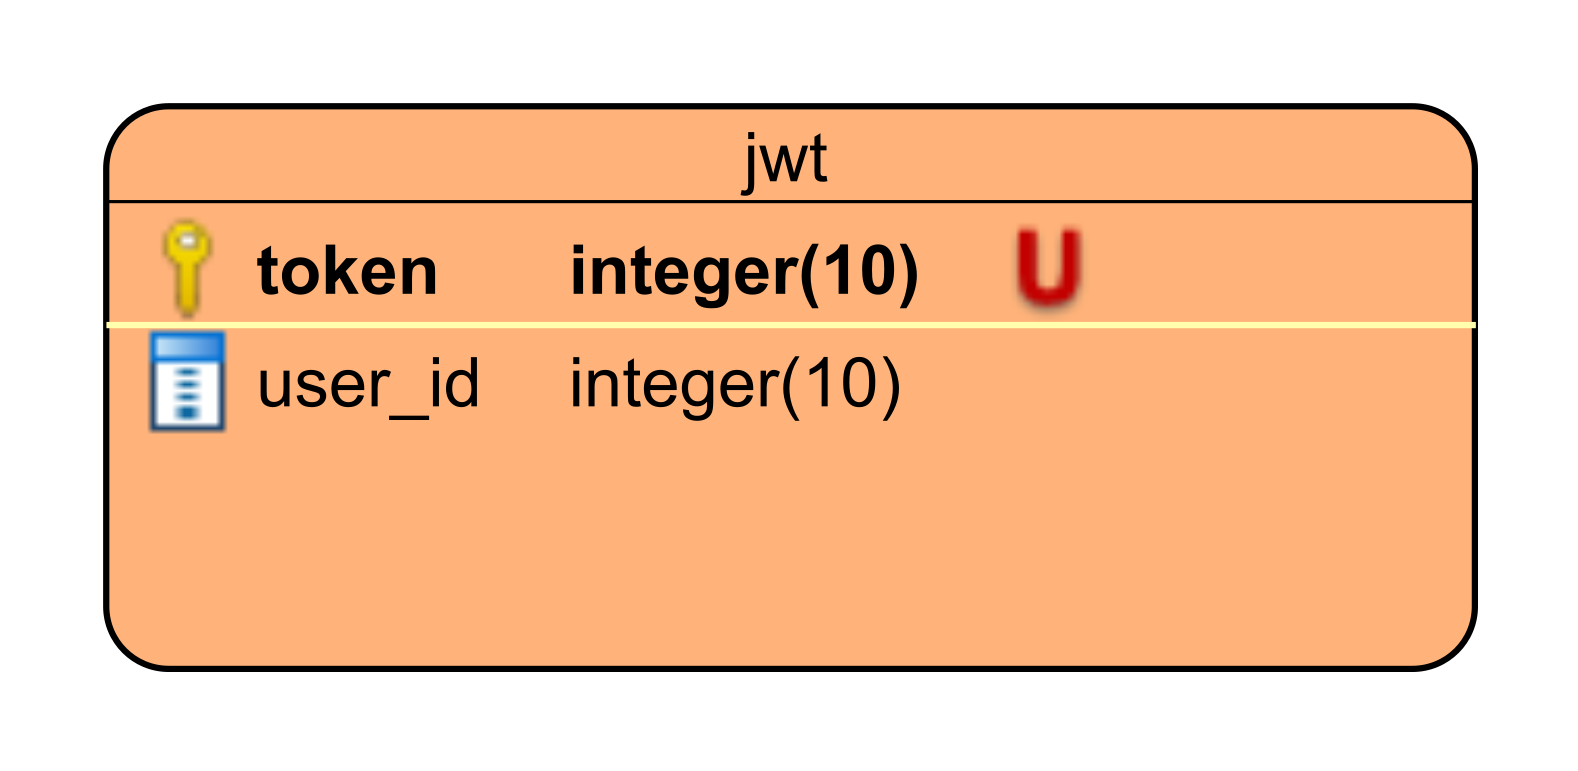
\includegraphics[width=6cm]{Figures/P3/DataModelAuth.png}
\end{center}
\subsubsection{Microservicio chat}
En esta vista, el microservicio de chat almacena información del usuario que envia el mensaje, a que sala de chat lo envía, el mensaje, y si este mensaje será oculto (el usuario decidió eliminarlo). También se guarda la hora en el que el mensaje fue enviado.
\begin{center}
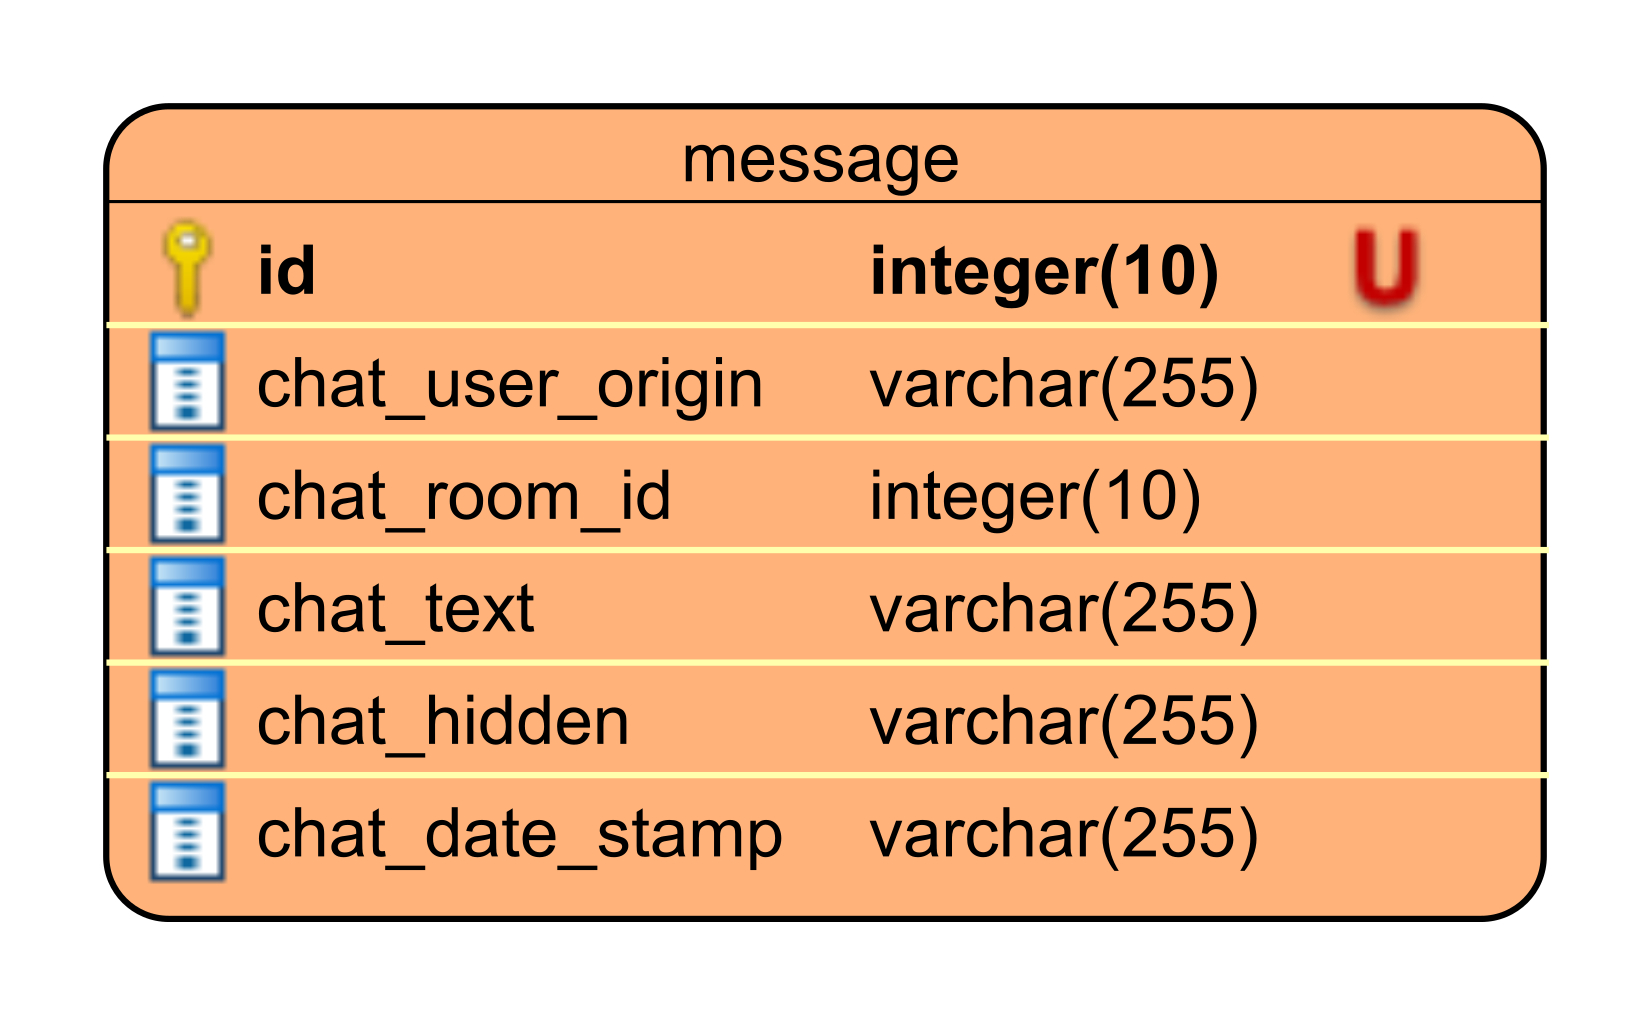
\includegraphics[width=6cm]{Figures/P3/DataModelChat.png}
\end{center}
\subsubsection{Microservicio chat-rooms}
Los chat-room almacenan información referentes a las salas de chat como lo son el nombre de la sala y qué usuarios pertenecen a élla. Esta entidad puede ser ampliada para contener mas información.
\begin{center}
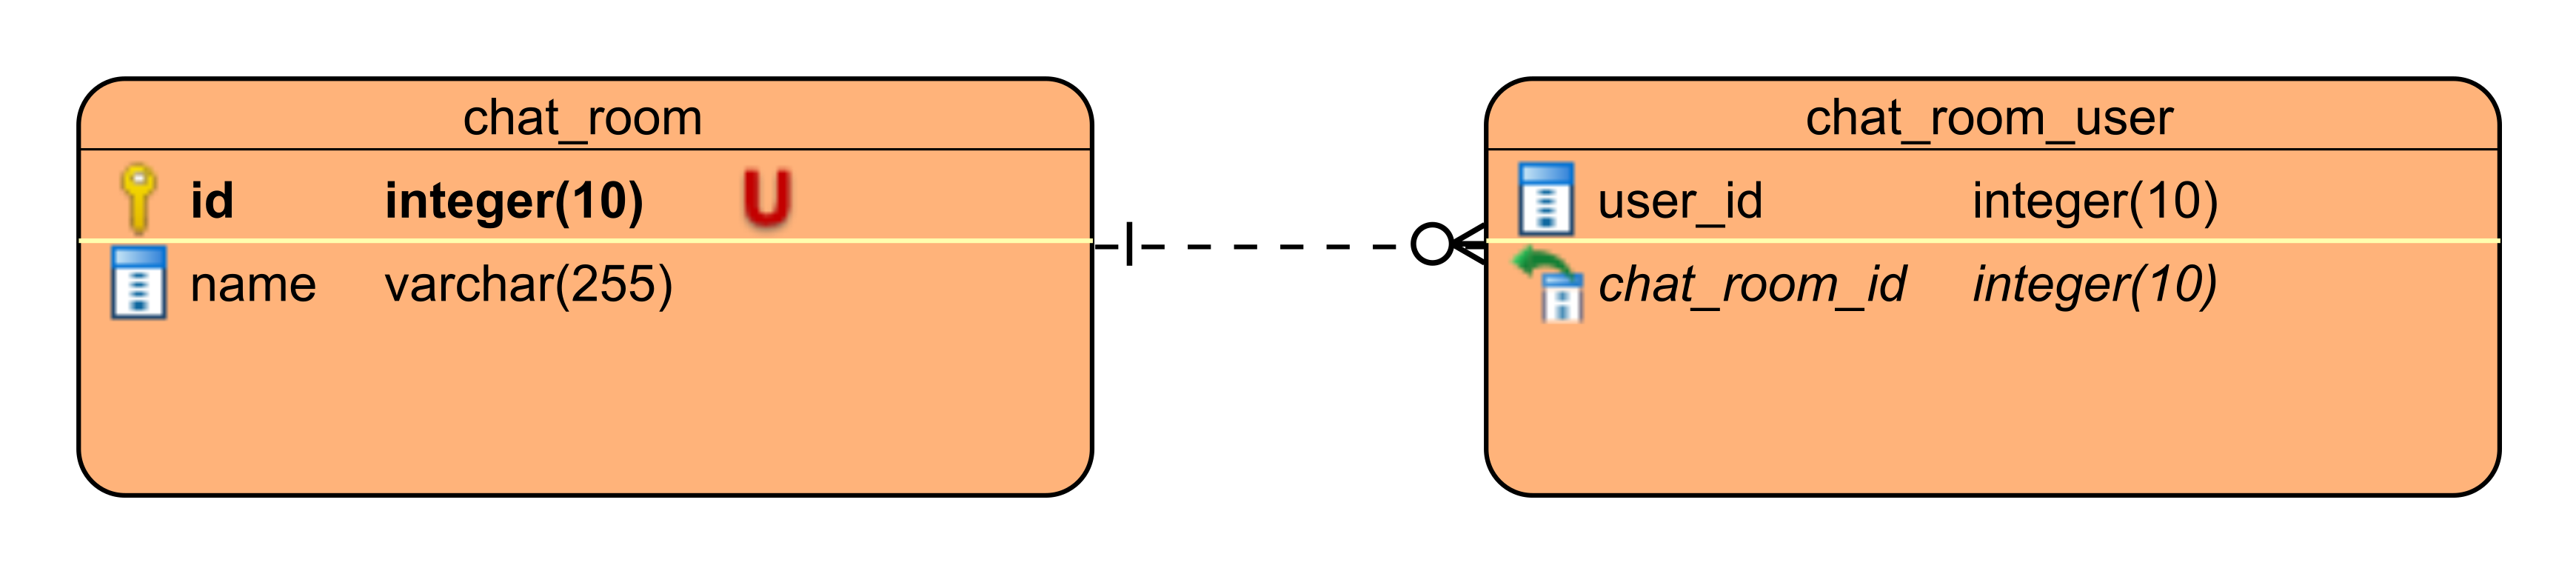
\includegraphics[width=8cm]{Figures/P3/DataModelChatroom.png}    
\end{center}
\subsubsection{Microservicio notificaciones}
Para las notificaciones, es de interés guardar información sobre los dispositivos que usan los usuarios, además de la información de las notificaciones en si tal como qué usuario es el que le hace llegar la notificación, el título y el mensaje de esta.
\begin{center}
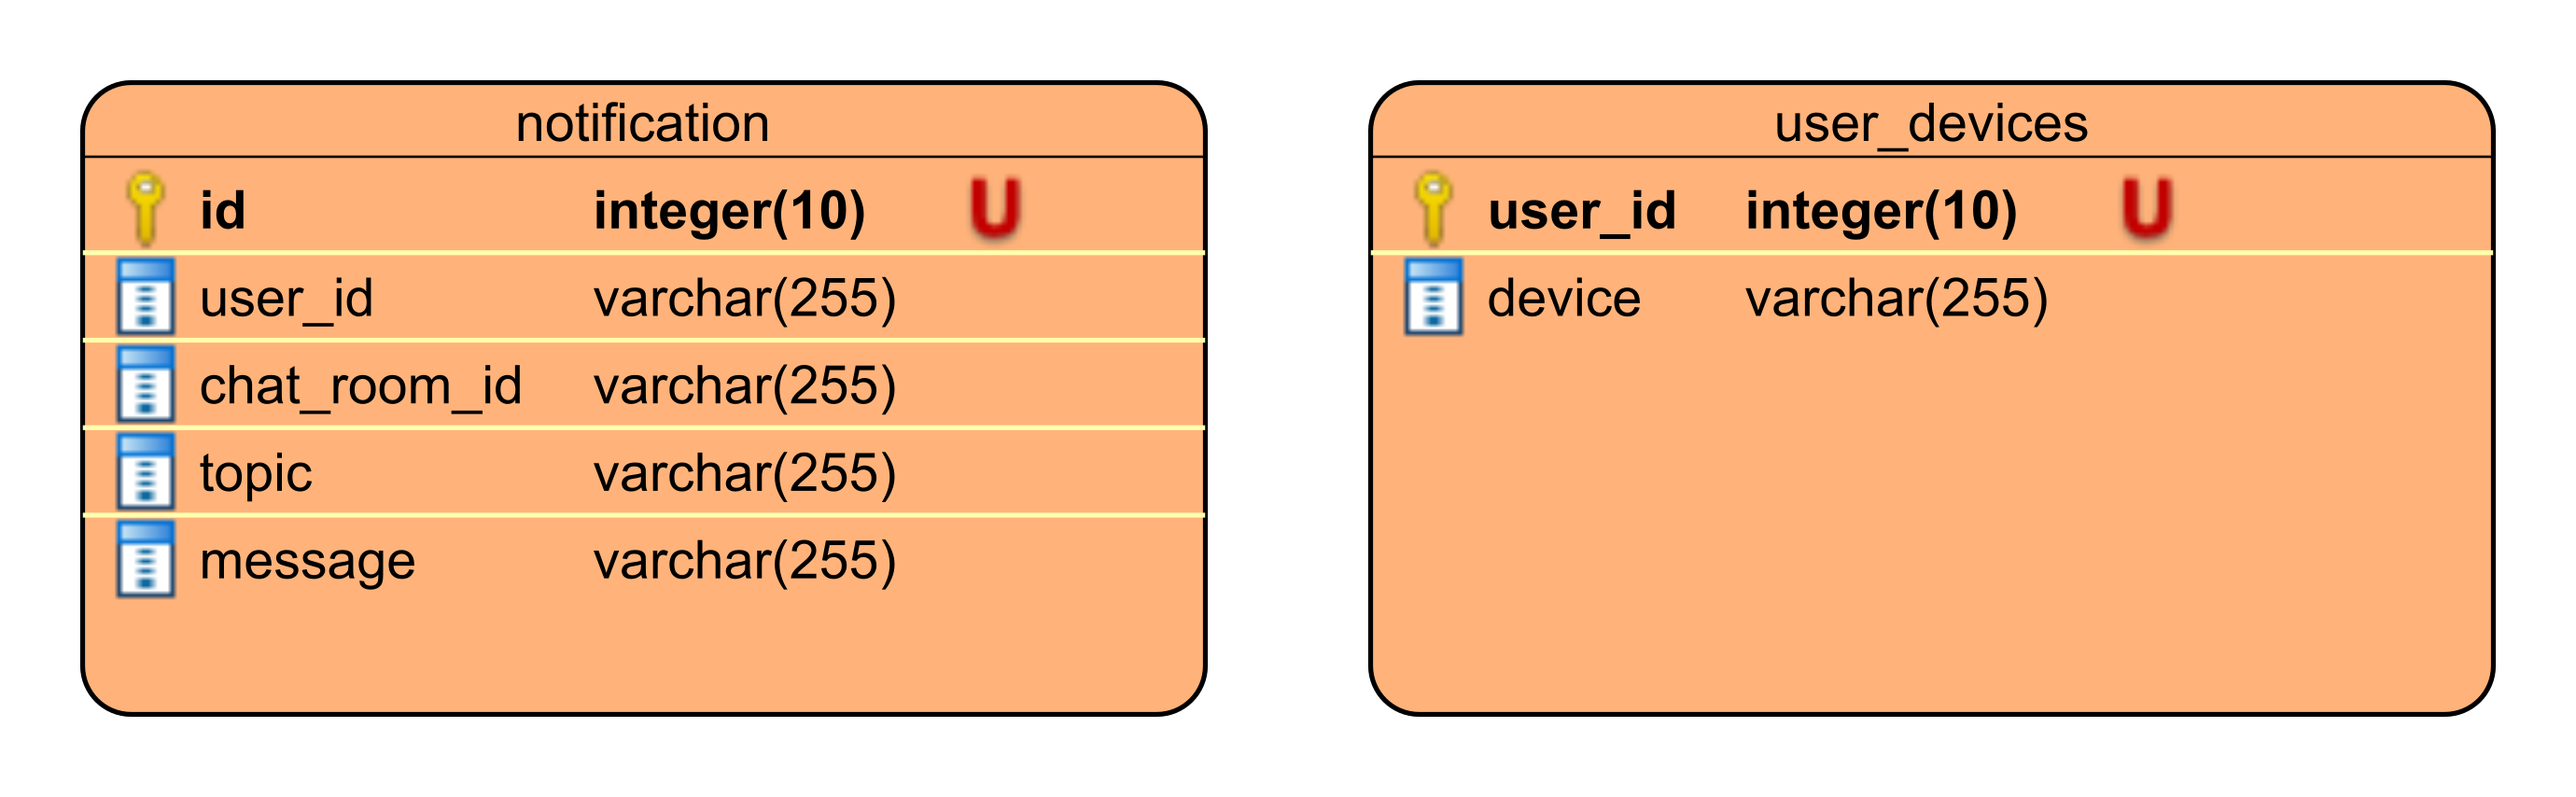
\includegraphics[width=8cm]{Figures/P3/DataModelNotifications.png}        
\end{center}
\subsection{Vista de Componentes y Conectores}
Para explicar el diagrama de componentes se listarán los componentes usados, junto la explicación de su uso, además de la lista de sus relaciones.
\begin{itemize}
    \item Componente de kwii\textunderscore api\\
    Es el componente que se encargará de orquestar los servicios ofrecidos por la plataforma.\\
    Los elementos con los que se relaciona utilizando conectores REST son:
    \begin{itemize}
        \item El componente de User-ms:\\
        Para poder orquestar el manejo de usuarios.
        \item El componente de Autentication-ms:\\
        Para poder orquestar el manejo de sesiones y autenticación de la aplicación.
        \item El componente de Chat-ms:\\
        Para orquestar el envío de chats en la aplicación.
        \item El componente de Chatroom-ms:\\
        Para orquestar la creación de los diversos chats.
        \item El componente de Notification-ms:\\
        Para orquestar el envío de notificaciones a los usuarios.
        \item El componente de kwii\textunderscore interface:\\
        Para orquestar el consumo de otras plataformas.
    \end{itemize}
    Los elementos con los que se relaciona utilizando conectores GraphQL son:
    \begin{itemize}
        \item El componente de kwii-proxy:\\
        Para poder exponer los servicios de la plataforma por medio del proxy inverso.
        \item El componente de kwii\textunderscore interface:\\
        Para exponer los servicios de la Kwii Platform a otras plataformas.
    \end{itemize}
    \item Componente de User-ms\\
    Este es el componente que manejará la información de los usuarios, pero poco tendrá que ver con el manejo de sus contraseñas.
    Este componente se relaciona con los siguientes:
    \begin{itemize}
        \item El componente User-db por medio del conector pg:\\
        Para almacenar los datos sobre los usuarios.
        \item El componente kwii \textunderscore api por medio de un conector REST:\\
        Para exponer los servicios de los usurios a través de él.
        \item El componente kwii \textunderscore ldpa por medio de un conector LDAP:\\
        Para guardar información de los usuarios en un directorio.
    \end{itemize}
    \item Componente User-db
    Este componente almacenará la información de los usuarios y las amistades de los usuarios.
    Los componentes que se relacionan con la base de datos de los usuarios son:
    \begin{itemize}
        \item El componente User por medio del conector pg:\\
        Para poder ofrecer los servicios de los usuarios.
        \item El componente Autentication por medio del conector pg node:\\
        Para adquirir las contraseñas de los usuarios.
    \end{itemize}
    \item Componente Autenticación-ms:\\
    El componente de Autenticación-ms será el encargado del manejo de sesiones dentro de la aplicación.
    Las relaciones de este componente son:
    \begin{itemize}
        \item El componente kwii \textunderscore api por medio de un conector REST:\\
        Para exponer los servicios de la autenticación a través de él.
        \item El componente de User-db por medio del conector pg node:\\
        Para poder recuperar las contraseñas de los usuarios de la base de datos.
        \item El componente de kwii-ldap por medio del conector LDAP:\\
        Para poder verificar que sean correctas las contraseñas de los usuarios por medio del LDAP.
        \item El componente de Autentication-db por medio del conector ioredis:\\
        Para poder usar almacenar información de User DB en cache.
    \end{itemize}
    \item Componente de Autentication-db:\\
     Las contraseñas son almacenadas en caché para evitar el uso de la base de datos User DB y la verificación del JWT usando la base de datos de Usuarios.\\
     Los componentes que se comunican con él son:
     \begin{itemize}
        \item El componente de Autentication-ms por medio del conector ioredis:\\
        Para poder usar la información de usuarios almacenada en caché
    \end{itemize}
    \item Componente Chat-ms:\\
    Es el componente encargado del tránsito de la gestión de los mensajes en el sistema.\\
    Los componentes con los que se comunica son:
    \begin{itemize}
        \item El componente kwii\textunderscore api por medio de un conector REST:\\
        Para exponer los servicios de la gestión de los mensajes a través de él.
        \item El componente Chat-db por medio del conector mongoengine:\\
        Es usado para almacenar los mensajes en una base orientada a documentos NoSQL.
    \end{itemize}
    \item Componente Chat-db\\
    Es el componente que almacena los mensajes en el sistema.\\
    Los componentes con los que se comunica son:
    \begin{itemize}
        \item El componente Chat-ms por medio del conector mongoengine:\\
        El componente chat utilizará chat DB  para almacenar los mensajes.
    \end{itemize}
    \item Componente Chatroom-ms\\
    Es el componente que gestiona las salas de chat, donde los usuarios podrán enviar mensajes.
    Los componentes con los que se comunica son:
    \begin{itemize}
        \item El componente kwii\textunderscore api por medio de un conector REST:\\
        Para exponer los servicios de la gestión de las salas de usuario a través de él.
        \item El componente Chatroom-db por medio del conector jdbc:\\
        Para almacenar la infomación relacionada con las salas de chats.
    \end{itemize}
    \item Componente Chatroom-db\\
    Es el componente que almacena la información relacionada con las salas de chat.
    Los componentes con los que se comunica son:
    \begin{itemize}
        \item El componente Chatroom-ms por medio del conector jdbc:\\
        El componente Chatroom-ms utilizará ChatRoom DB para almacenar la infomación relacionada con las salas de chats.
    \end{itemize}
    \item Componente Notification-ms\\
    Es el componente que administra las notificaiones hacia los usuarios en el sistema.
    Los componentes con los que se comunica son:
    \begin{itemize}
        \item El componente kwii\textunderscore api por medio de un conector REST:\\
        Para exponer los servicios de la gestión de notificaiones a través de él.
        \item El componente Notification-db por medio del conector go\textunderscore redis:\\
        Para almacenar la infomación relacionada con las notificaciones.
    \end{itemize}
    \item Componente Notification-db\\
    Es el componente que almacena la información relacionada con las notificaiones en el sistema.
    Los componentes con los que se comunica son:
    \begin{itemize}
        \item El componente Notification-ms por medio del conector go\textunderscore redis:\\
        El componente Notification-ms utilizará Notification-db para almacenar la infomación relacionada con las notificaciones.
    \end{itemize}
    \item Componente kwii-proxy:\\
    Es el componente encargado de exponer los servicios de la Kwii Platform:\\
    Los componentes con los que se comunica son:
    \begin{itemize}
        \item El componente kwii-wa por medio del conector REST:\\
        Para exponer los servicios de la Kwii Platform para los usuarios web.
        \item El componente kwii-ma por medio del conector REST:\\
        Para exponer los servicios de la Kwii Platform para los usuarios mobile.
    \end{itemize}
    \item Componente kwii-wa:\\
    Es el componente encargado de consumir los servicios expuestos por el kwii\textunderscore api por medio del kwii-proxy para la presentación al usuario por medio de la web:\\
    Los componentes con los que se comunica son:
    \begin{itemize}
        \item El componente kwii\textunderscore proxy por medio del conector REST:\\
        Para consumir los servicios expuestos por el kwii-api.
    \end{itemize}
    \item Componente kwii-ma:\\
    Es el componente encargado de consumir los servicios expuestos por el kwii\textunderscore api por medio del kwii-proxy para la presentación al usuario de una aplicación móvil:\\
    Los componentes con los que se comunica son:
    \begin{itemize}
        \item El componente kwii\textunderscore proxy por medio del conector REST:\\
        Para consumir los servicios expuestos por el kwii-api.
    \end{itemize}
\end{itemize}
\begin{center}
    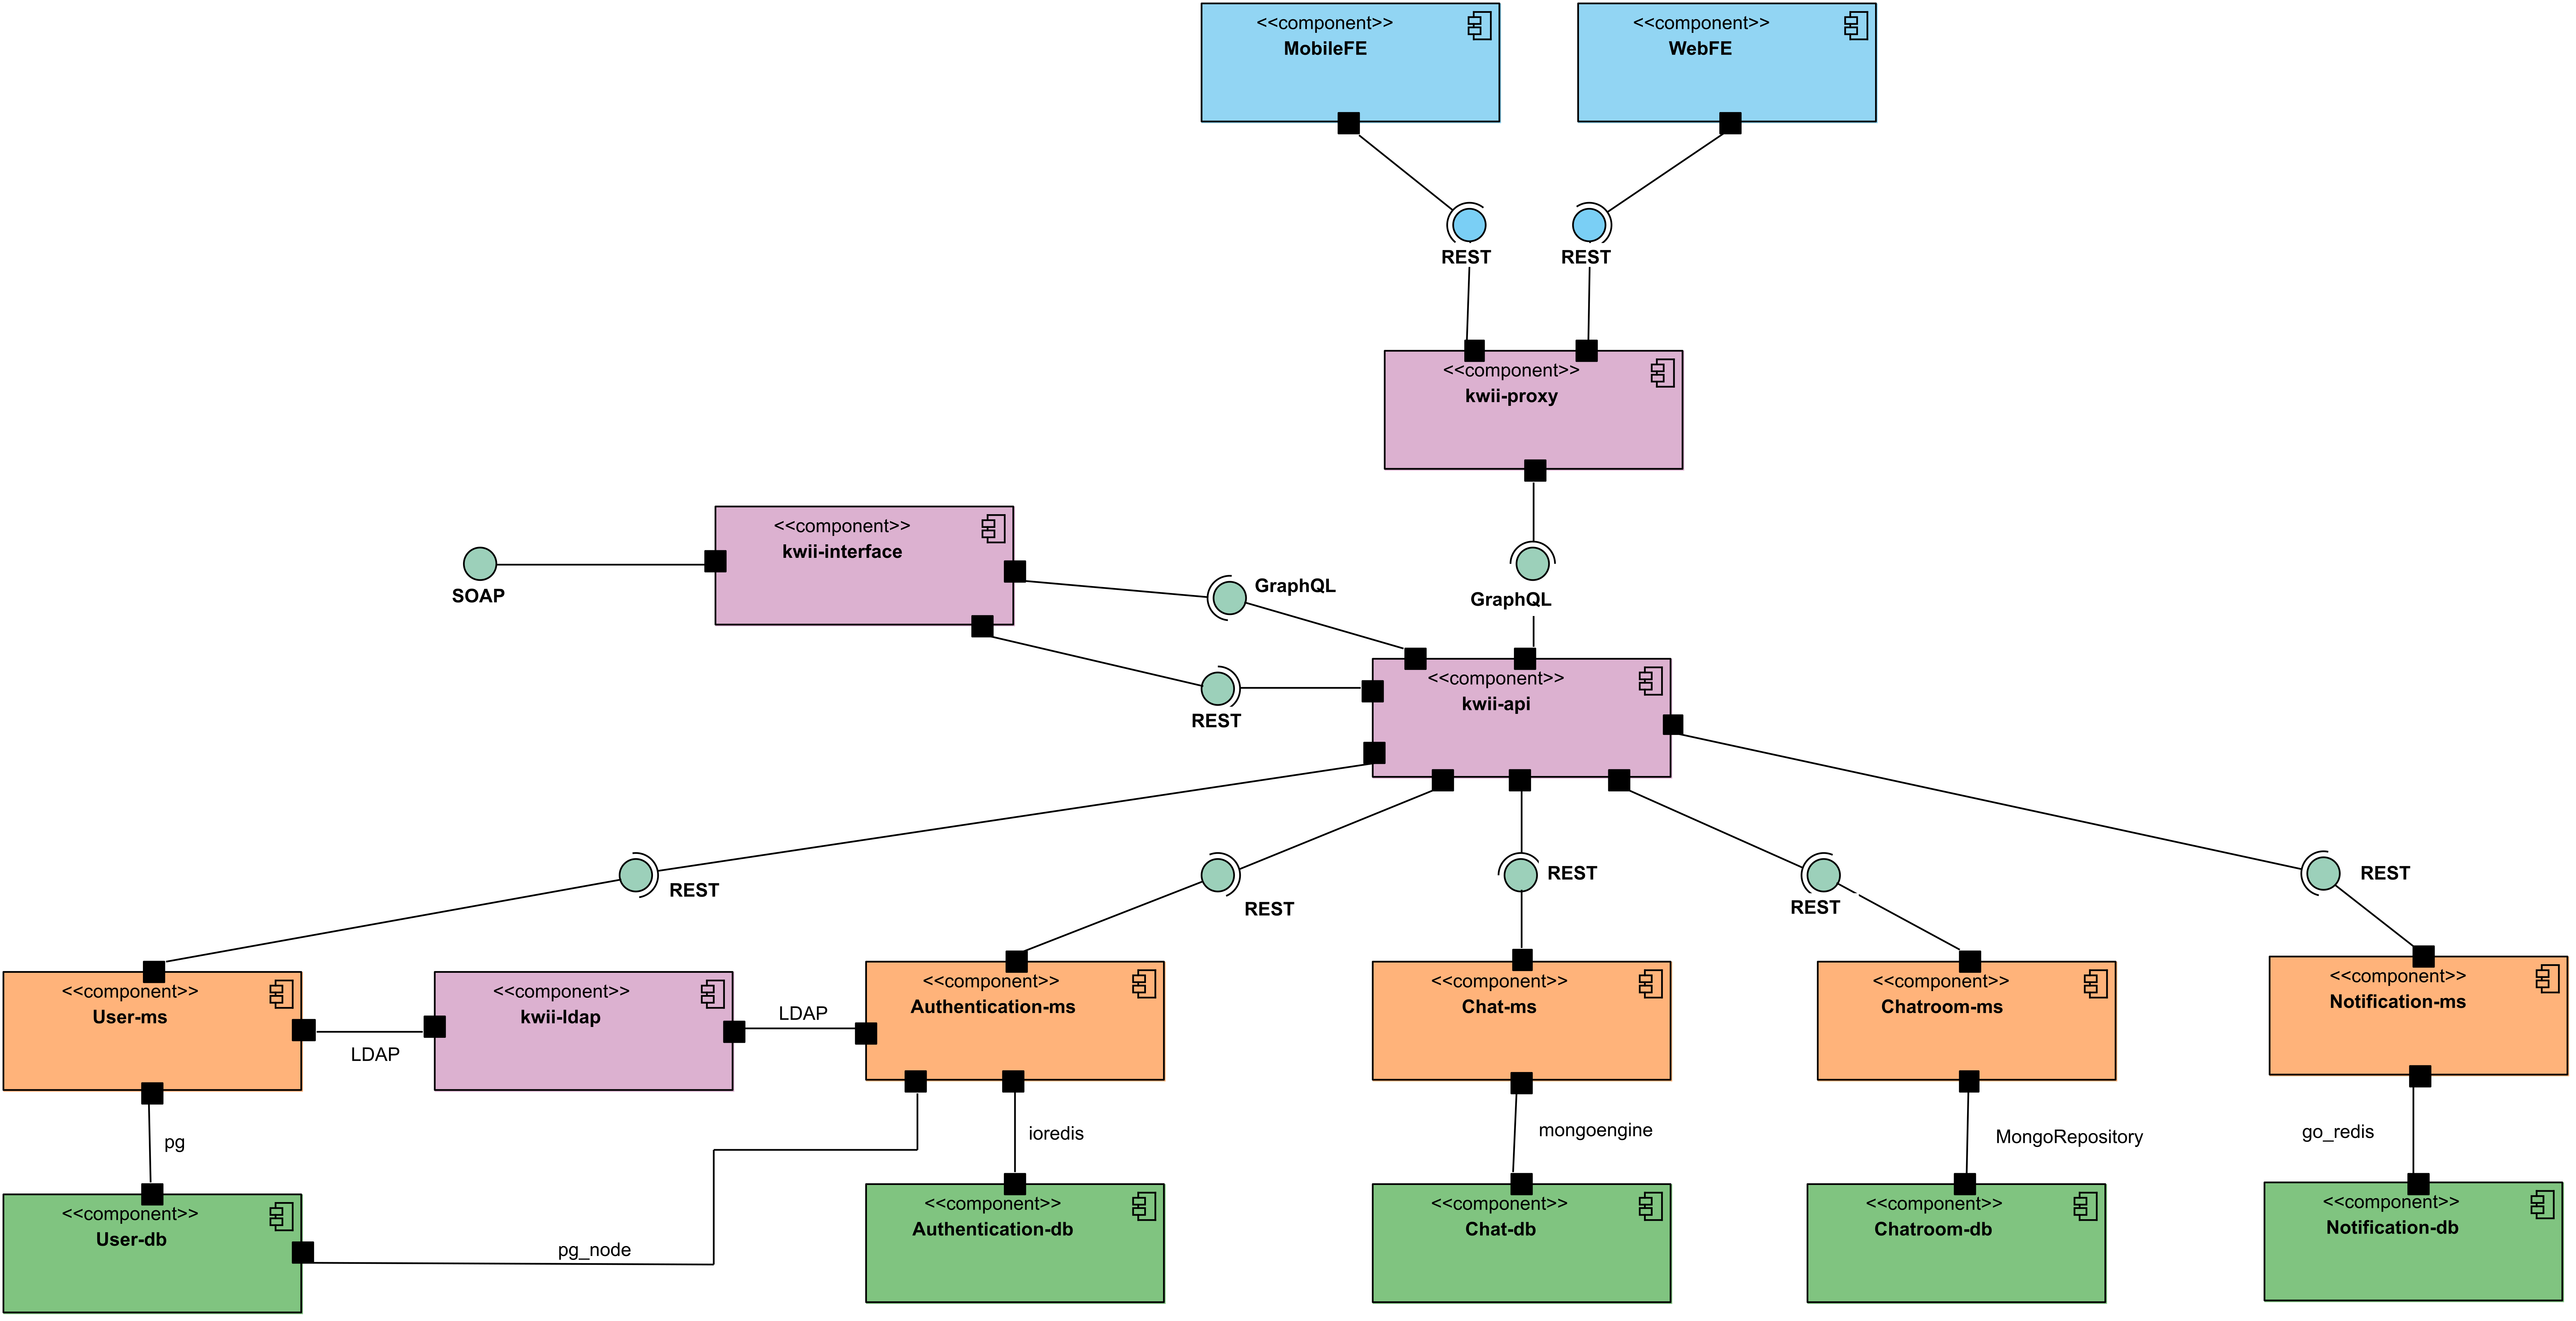
\includegraphics[width=14cm]{Figures/P3/CYC.png}    
\end{center}

\subsection{Vista de Capas}
La vista de capas nos permite visualizar de manera precisa la secuencia lógica por la que pasa la información en la aplicación, para presentar esta vista se ha divido en 3 tiers los cuales son:\\

\begin{itemize}
    \item Presentacion: \\
    El tier de presentación es el más cercano al usuario final y está compuesto por 2 capas las cuales componen el Front End de la aplicación (Web FrontEnd y Mobile FrontEnd). \\
    Ambas capas tienen permitido acceder al tier de lógica haciendo uso de la capa del proxy inverso.
    \item lógica: \\
    El tier  de lógica contiene, como su nombre lo indica, toda la lógica de la obtención y manipulación de los datos usados por la aplicación, este tier está compuesto por las siguientes capas: \\
    \begin{itemize}
        \item kwii-proxy \\
        Recibe y encamina los datos recibidos por los FrontEnd hacia el kwii\textunderscore api. 
        \item orchestation
        La capa orchestation se refiere al uso de los microservicios para el consumo de los microservicios y exposición de servicios más complejos. Y además, el consumo de plataformas externas.
        La capa de orchestation tiene:
        \begin{itemize}
            \item Api-gateway \\
            Recibe y encamina los datos recibidos por los FrontEnd hacia las capas más internas, para esto se divide en 2 segmentos: 
            \begin{itemize}
                \item Esquema: \\
                Da formato a los datos recibidos haciendo uso del segmento de definición de tipos (type\_def) y los remite hacia el segmento de resolvers. 
                \item Modelo: \\
                El segmento de modelo encierra a su vez 3 segmentos especializados, el esquema, que puede usar los resolvers y los type\textunderscore def, y los resolvers pueden usar los servidores.
            \end{itemize}
            \item kwii-interface
            Recibe y trata solicitudes de otras plataformas. Es un segmento de capa de la orchestation.
        \end{itemize}
        \item Users-ms \\
        Recibe las peticiones relacionadas a la administracion de usuarios, este componente da respuesta a las solicitudes haciendolas pasar por 3 segmentos:
        \begin{itemize}
            \item View: \\
            Expone la ruta y define los parametros necesarios para una accion concreta.
            \item Controller: \\
            Lleva a cabo la operaciones especificas para poder cumplir con la solicitud.
            \item Model: \\
            Expresa los atributos e informacion necesaria que tiene cada uno de los datos para poder ser operados, es la capa lógica mas cercana a los datos en bruto.
        \end{itemize}
        
        \item Notifications-ms \\
        Recibe las peticiones e información necesaria para poder realizar el envio de notificaciones a los usuario, el flujo de esta informacion pasa por los siguiente segmentos:
        \begin{itemize}
            \item View: \\
            Expone la ruta y define los parametros necesarios para una accion concreta.
            \item Controller: \\
            Lleva a cabo la operaciones especificas para poder cumplir con la solicitud.
            \item Model: \\
            Expresa los atributos e informacion necesaria que tiene cada uno de los datos para poder ser operados, es la capa lógica mas cercana a los datos en bruto.
        \end{itemize}
        
        \item Authentication-ms \\
        Recibe las peticiones relacionadas a la autenticacion de usuarios, este componente da respuesta a las solicitudes haciendolas pasar por 2 segmentos:
        \begin{itemize}
            \item View: \\
            Expone la ruta y define los parametros necesarios para una accion concreta.
            \item Controller: \\
            Lleva a cabo la operaciones especificas para poder cumplir con la solicitud.
            \item Model: \\
            Expresa los atributos e informacion necesaria que tiene cada uno de los datos para poder ser operados, es la capa lógica mas cercana a los datos en bruto.
        \end{itemize}
        
        \item Chatroom-ms \\
        Recibe las peticiones relacionadas a la administracion de salas de chat, este componente da respuesta a las solicitudes haciendolas pasar por 3 segmentos:
        \begin{itemize}
            \item View: \\
            Expone la ruta y define los parametros necesarios para una accion concreta.
            \item Controller: \\
            Lleva a cabo la operaciones especificas para poder cumplir con la solicitud.
            \item Model: \\
            Expresa los atributos e informacion necesaria que tiene cada uno de los datos para poder ser operados, es la capa lógica mas cercana a los datos en bruto.
        \end{itemize}
        
        \item Chat-ms \\
        Recibe las peticiones relacionadas a los mensajes que se dan en los chats, este componente da respuesta a las solicitudes haciendolas pasar por 3 segmentos:
        \begin{itemize}
            \item View: \\
            Expone la ruta y define los parametros necesarios para una accion concreta.
            \item Controller: \\
            Lleva a cabo la operaciones especificas para poder cumplir con la solicitud.
            \item Model: \\
            Expresa los atributos e informacion necesaria que tiene cada uno de los datos para poder ser operados, es la capa lógica mas cercana a los datos en bruto.
        \end{itemize}
        
    \end{itemize}
    
    \item Datos: \\
    Es el tier mas alejado de el usuario final, contine un capa de base de datos en donde los diferentes modelos de la aplicación extraen la informacion que necesitan.\\
    Esta capa a su vez tiene 5 segmentos correspondientes a cada uno de los microservicios, estos son:
    \begin{itemize}
        \item User DB
        \item Notifications DB
        \item Authentication DB
        \item Chat Room DB
        \item Chat DB
    \end{itemize}
    Además, contiene una capa de directorio, donde se guarda información fundamental de los usuarios.
\end{itemize}

\begin{center}
    \includegraphics[width=14cm]{Figures/P3/Layered.png}    
\end{center}

\subsection{Vista de Despliegue}
Para la vista de depliegue se tiene una máquina virtual que está ejecutando un ambiente Linux y es un nodo rancher. Esta máquina responde al host 34.73.50.226 y en él se despliegan los componentes de la aplicación en contenedores de la siguiente manera:
\begin{itemize}
    \item Un contenedor con el ambiente de ejecución Nginx que expone el puerto 443 para el despliegue del componente kwii-proxy.
    \item Un contenedor con el ambiente de ejecución Python que expone el puerto 8420 para el despliegue del componente kwii-interface.
    \item Un contenedor con el ambiente de ejecución Ruby que expone el puerto 3000 para el despliegue del componente User.
    \item Un contenedor con el ambiente de ejecución Postgres que expone el puerto 5432 para el despliegue del componente User DB.
    \item Un contenedor con el ambiente de ejecución TomEE que expone el puerto 4000 para el despliegue del componente ChatRoom.
    \item Un contenedor con el ambiente de ejecución MySQL que expone el puerto 3306 para el despliegue del componente ChatRoom DB.
    \item Un contenedor con el ambiente de ejecución Python que expone el puerto 8000 para el despliegue del componente Chat.
    \item Un contenedor con el ambiente de ejecución MongoDB que expone el puerto 27017 para el despliegue del componente Chat DB.
    \item Un contenedor con el ambiente de ejecución NodeJS que expone el puerto 3200 para el despliegue del componente Authentication.
    \item Un contenedor con el ambiente de ejecución Redis que expone el puerto 6379 para el despliegue del componente Authentication DB.
    \item Un contenedor con el ambiente de ejecución Go que expone el puerto 9000 para el despliegue del componente Notification.
    \item Un contenedor con el ambiente de ejecución Redis que expone el puerto 9001 para el despliegue del componente Notification DB.
    \item Un contenedor con el ambiente de ejecución NodeJS que expone el puerto 5500 para el despliegue del componente api\textunderscore gateway.
\end{itemize}
\begin{center}
    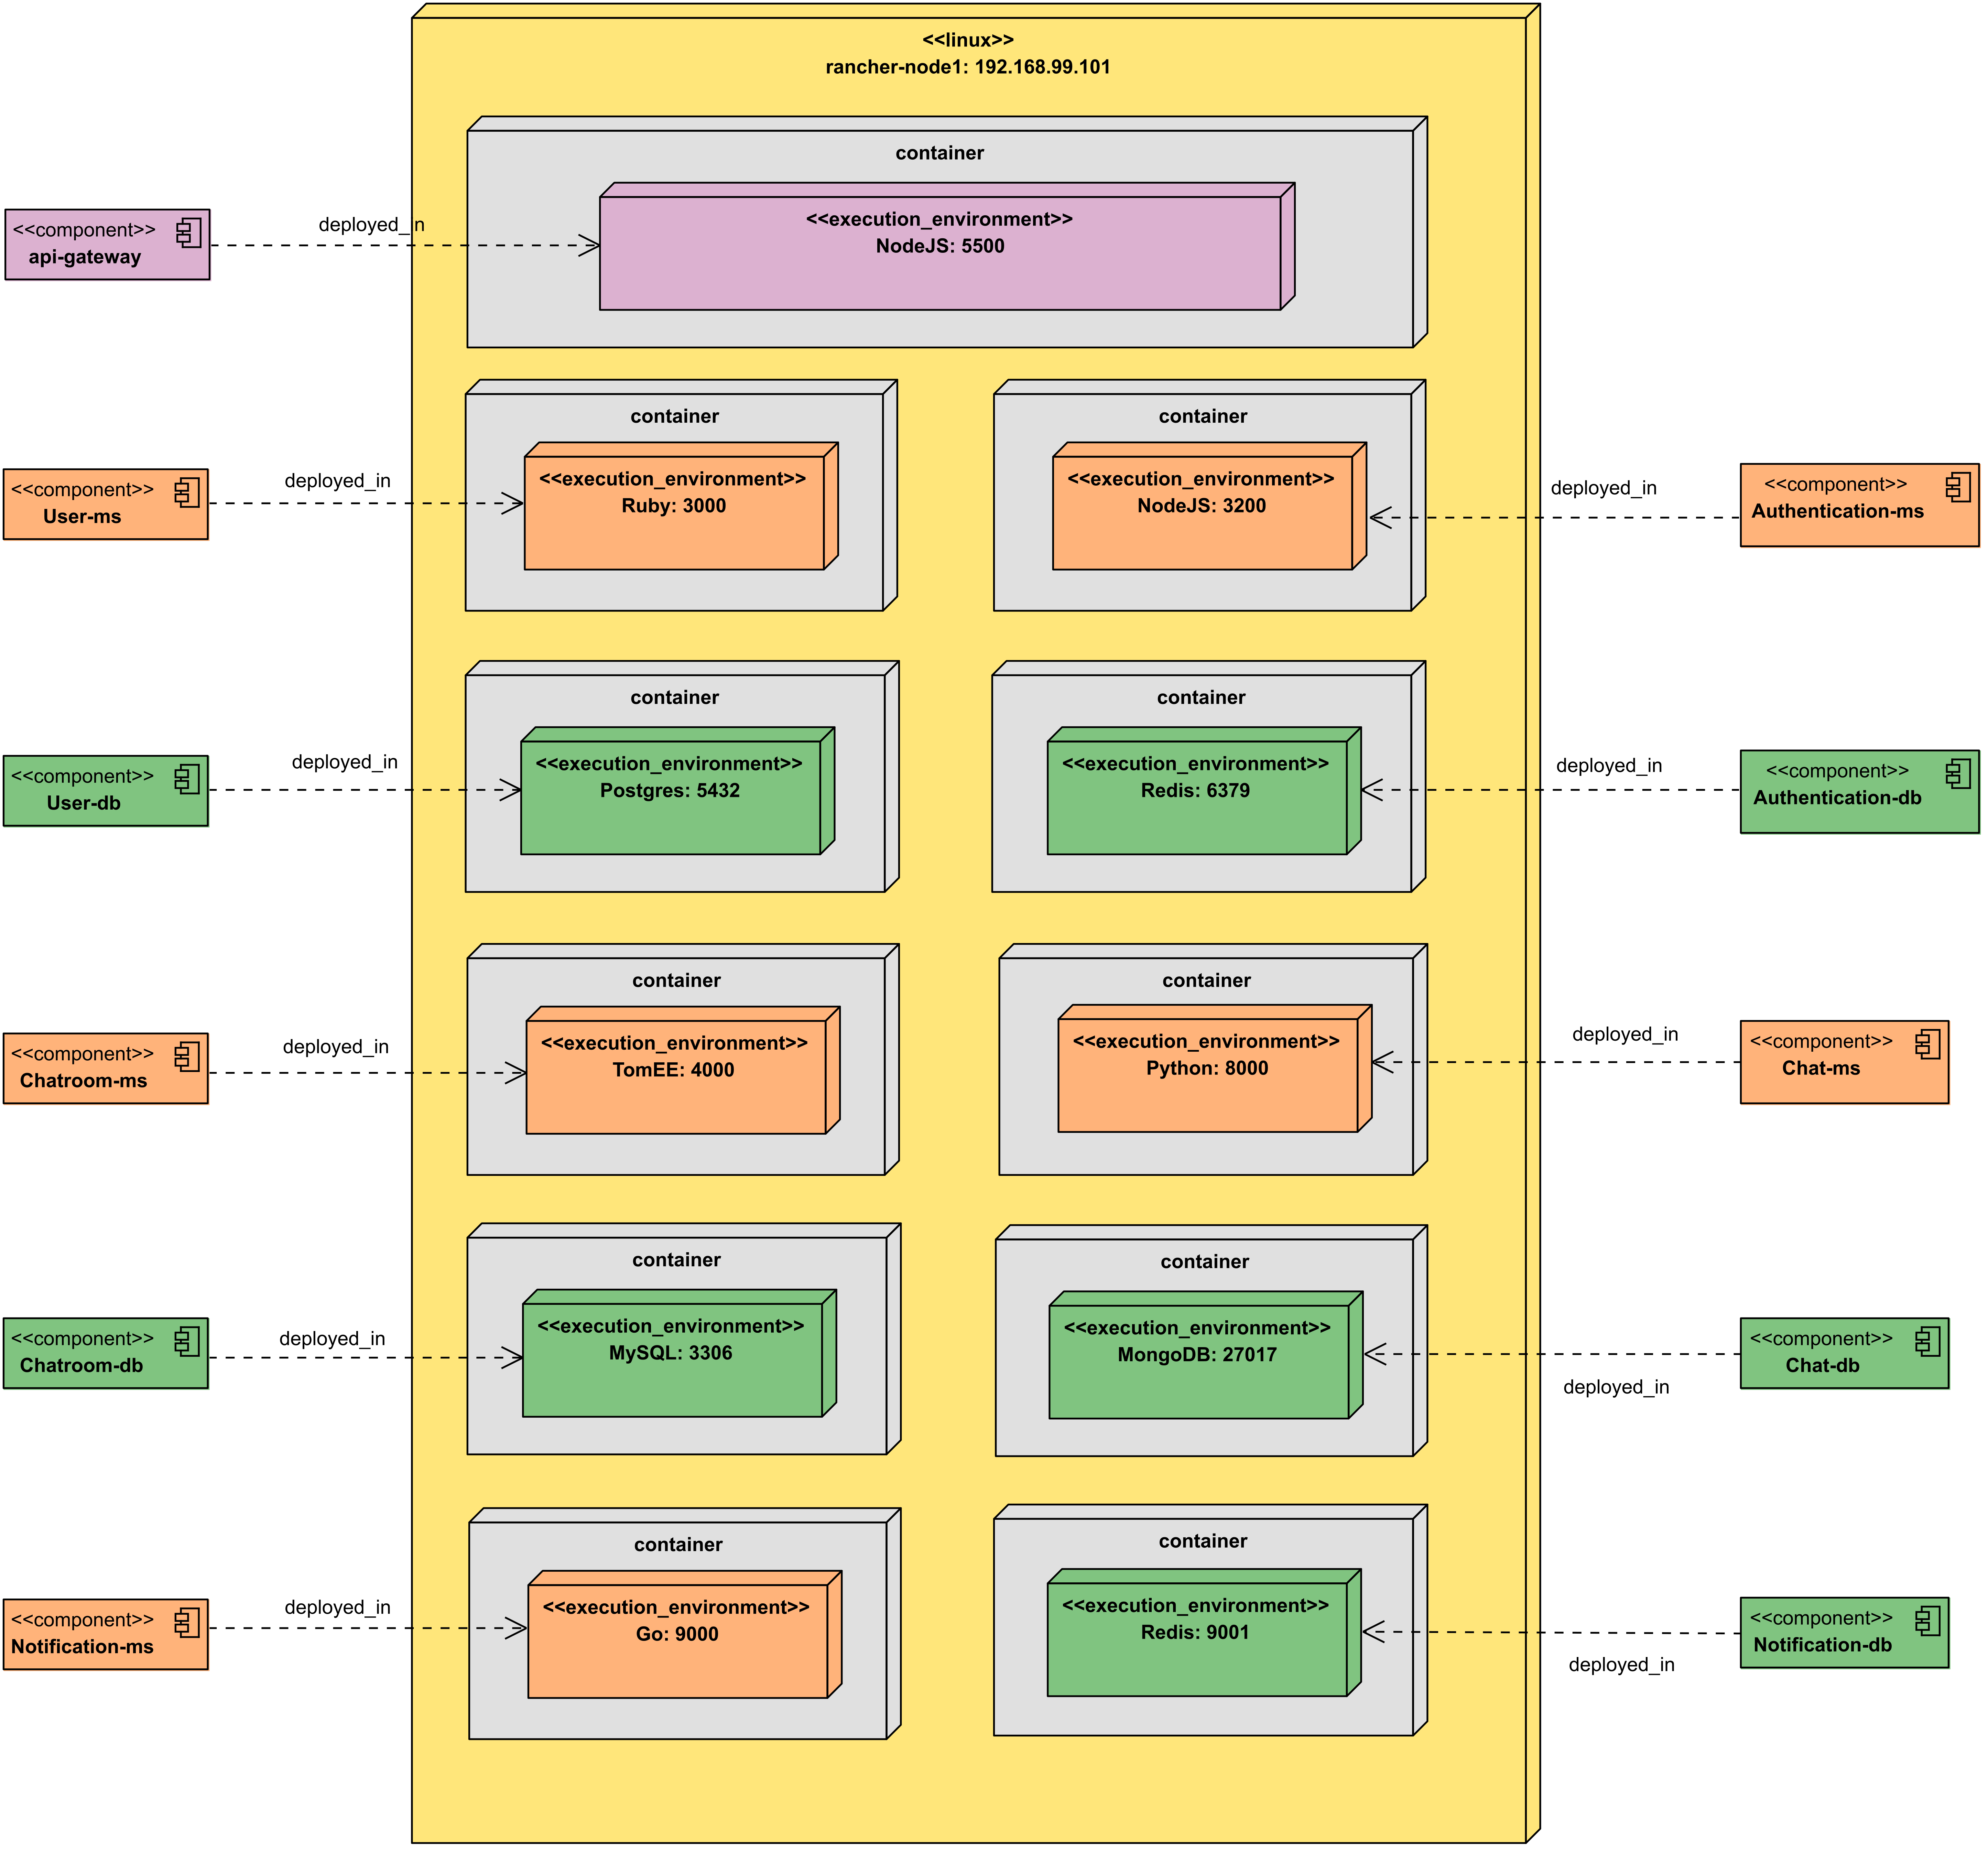
\includegraphics[width=15cm,height=20cm,keepaspectratio]{Figures/P3/deployment.png}    
\end{center}